\documentclass[conference]{IEEEtran}
% QONTOS Research Paper Series — Shared LaTeX Preamble
% Use with: % QONTOS Research Paper Series — Shared LaTeX Preamble
% Use with: % QONTOS Research Paper Series — Shared LaTeX Preamble
% Use with: \input{qontos-preamble}

\usepackage{cite}
\usepackage{amsmath,amssymb,amsfonts}
\usepackage{graphicx}
\usepackage{textcomp}
\usepackage{xcolor}
\usepackage{hyperref}
\usepackage{booktabs}
\usepackage{multirow}
\usepackage{array}
\usepackage{tabularx}
\usepackage{float}
\usepackage{listings}
\usepackage{url}
\usepackage{enumitem}

% Listing style
\lstset{
  basicstyle=\ttfamily\footnotesize,
  breaklines=true,
  frame=single,
  backgroundcolor=\color{gray!10},
}

% Custom column type
\newcolumntype{L}[1]{>{\raggedright\arraybackslash}p{#1}}

% QONTOS colors
\definecolor{qontosnavy}{HTML}{0A1628}
\definecolor{qontosblue}{HTML}{1E88E5}
\definecolor{qontosteal}{HTML}{00BCD4}

% Hyperref setup
\hypersetup{
  colorlinks=true,
  linkcolor=qontosblue,
  citecolor=qontosblue,
  urlcolor=qontosteal,
}

% Author block
\newcommand{\qontosauthor}{%
\IEEEauthorblockN{QONTOS Research Wing}
\IEEEauthorblockA{
Zhyra Quantum Research Institute (ZQRI)\\
Advanced Quantum Systems Division\\
Abu Dhabi, UAE\\
\texttt{research@zhyra.xyz}}
}


\usepackage{cite}
\usepackage{amsmath,amssymb,amsfonts}
\usepackage{graphicx}
\usepackage{textcomp}
\usepackage{xcolor}
\usepackage{hyperref}
\usepackage{booktabs}
\usepackage{multirow}
\usepackage{array}
\usepackage{tabularx}
\usepackage{float}
\usepackage{listings}
\usepackage{url}
\usepackage{enumitem}

% Listing style
\lstset{
  basicstyle=\ttfamily\footnotesize,
  breaklines=true,
  frame=single,
  backgroundcolor=\color{gray!10},
}

% Custom column type
\newcolumntype{L}[1]{>{\raggedright\arraybackslash}p{#1}}

% QONTOS colors
\definecolor{qontosnavy}{HTML}{0A1628}
\definecolor{qontosblue}{HTML}{1E88E5}
\definecolor{qontosteal}{HTML}{00BCD4}

% Hyperref setup
\hypersetup{
  colorlinks=true,
  linkcolor=qontosblue,
  citecolor=qontosblue,
  urlcolor=qontosteal,
}

% Author block
\newcommand{\qontosauthor}{%
\IEEEauthorblockN{QONTOS Research Wing}
\IEEEauthorblockA{
Zhyra Quantum Research Institute (ZQRI)\\
Advanced Quantum Systems Division\\
Abu Dhabi, UAE\\
\texttt{research@zhyra.xyz}}
}


\usepackage{cite}
\usepackage{amsmath,amssymb,amsfonts}
\usepackage{graphicx}
\usepackage{textcomp}
\usepackage{xcolor}
\usepackage{hyperref}
\usepackage{booktabs}
\usepackage{multirow}
\usepackage{array}
\usepackage{tabularx}
\usepackage{float}
\usepackage{listings}
\usepackage{url}
\usepackage{enumitem}

% Listing style
\lstset{
  basicstyle=\ttfamily\footnotesize,
  breaklines=true,
  frame=single,
  backgroundcolor=\color{gray!10},
}

% Custom column type
\newcolumntype{L}[1]{>{\raggedright\arraybackslash}p{#1}}

% QONTOS colors
\definecolor{qontosnavy}{HTML}{0A1628}
\definecolor{qontosblue}{HTML}{1E88E5}
\definecolor{qontosteal}{HTML}{00BCD4}

% Hyperref setup
\hypersetup{
  colorlinks=true,
  linkcolor=qontosblue,
  citecolor=qontosblue,
  urlcolor=qontosteal,
}

% Author block
\newcommand{\qontosauthor}{%
\IEEEauthorblockN{QONTOS Research Wing}
\IEEEauthorblockA{
Zhyra Quantum Research Institute (ZQRI)\\
Advanced Quantum Systems Division\\
Abu Dhabi, UAE\\
\texttt{research@zhyra.xyz}}
}


\begin{document}

\title{Benchmarking Framework for Large-Scale Modular Quantum Systems}
\author{\qontosauthor}
\maketitle

\begin{abstract}
Credible quantum computing programs require benchmark frameworks that distinguish measured results from architectural projections and aspirational targets. This paper defines the QONTOS benchmarking framework: a layered protocol suite that spans simulator-backed orchestration, digital-twin modeling, noisy baselines, and eventual fault-tolerant modular hardware. We specify exact benchmark definitions grounded in the peer-reviewed literature---including randomized benchmarking, Quantum Volume, CLOPS, and application-oriented suites---together with measurement conditions, confidence-interval reporting requirements, baseline comparisons, and pass/fail gating thresholds. The framework classifies every reported metric by its evidence level using mandatory claim labels and establishes a modular-system benchmarking methodology for the QONTOS hybrid superconducting-photonic architecture, covering both intra-module (superconducting) performance and cross-module (photonic) metrics such as inter-module gate fidelity and Bell pair generation rates. All protocols reference the open-source \texttt{qontos-benchmarks} repository as the canonical implementation. This paper serves as the credibility backbone of the QONTOS paper series: no claim in any companion paper is valid unless it maps to a benchmark, protocol, or validation gate defined here.

\textbf{Claim label:} METHODOLOGY---benchmark design, protocol specification, and release gating framework. No performance claims are made in this paper; all numeric values appearing in target tables carry explicit QONTOS-TARGET or STRETCH-TARGET labels.
\end{abstract}

\section{Introduction: Benchmarking as the Credibility Engine}

\subsection{Motivation and Scope}

The quantum computing field suffers from a credibility gap. Headline metrics are frequently reported without specifying measurement conditions, noise models, or the boundary between measured values and architectural projections. Proctor et al.\ (2022) demonstrated that even well-intentioned benchmark reporting can mislead when measurement protocols are underspecified~\cite{proctor2022}. Lubinski et al.\ (2023) further showed that application-oriented benchmarks require careful normalization to enable meaningful cross-platform comparison~\cite{lubinski2023}.

\textbf{[CLAIM-METHODOLOGY]} The QONTOS benchmarking framework addresses this gap by requiring every reported metric to carry: (a)~a claim label specifying its evidence basis, (b)~a complete measurement-condition record, (c)~at least one baseline comparison, and (d)~a confidence interval or explicit uncertainty statement.

This paper serves a structural role in the QONTOS paper series. Papers~01 through~08 and Paper~10 contain architectural claims, algorithm projections, and roadmap targets. None of those claims are valid in isolation. Each must trace to a benchmark definition, measurement protocol, or validation gate specified here. If a claim cannot be mapped to this framework, it must be labeled UNVALIDATED until a corresponding benchmark is defined.

\subsection{Claim Label Taxonomy}

Every metric, result, or projection reported in any QONTOS paper must carry exactly one of the following labels:

\begin{table}[H]
\centering
\caption{Claim label taxonomy.}
\label{tab:claim_labels}
\begin{tabular}{@{}l L{5.5cm}@{}}
\toprule
\textbf{Claim Label} & \textbf{Definition} \\
\midrule
MEASURED-SIMULATOR & Result obtained on the QONTOS simulator-backed pipeline \\
MEASURED-HARDWARE & Result obtained on physical quantum hardware \\
DIGITAL-TWIN-PROJECTION & Result from a calibrated noise model and modular runtime simulation \\
NOISY-BASELINE & Result from a standardized depolarizing or realistic noise channel \\
QONTOS-TARGET & Planned performance level under stated assumptions \\
STRETCH-TARGET & Aspirational performance level requiring multiple breakthroughs \\
LITERATURE-VALUE & Value taken from a published, peer-reviewed source \\
UNVALIDATED & Claim that does not yet map to a benchmark protocol \\
\bottomrule
\end{tabular}
\end{table}

\subsection{Benchmark Definitions}

This section defines the core benchmarks used throughout the QONTOS program, grounded in their original peer-reviewed specifications.

\textbf{Randomized Benchmarking (RB).} Introduced by Knill et al.\ (2008)~\cite{knill2008}, randomized benchmarking estimates average gate fidelity by measuring the decay of sequence fidelity as a function of the number of random Clifford gates applied to a qubit register. The protocol is efficient because the number of required sequences scales polynomially, and the result is largely independent of state-preparation and measurement (SPAM) errors. QONTOS adopts standard RB as the Layer-0 single-qubit and two-qubit gate characterization protocol.

\textbf{Interleaved Randomized Benchmarking (IRB).} Magesan et al.\ (2012)~\cite{magesan2012} extended RB to isolate the error rate of a specific gate by interleaving it between random Clifford operations. The ratio of the interleaved and reference decay rates yields the error per gate for the target operation. QONTOS uses IRB to characterize individual gate types---particularly cross-module entangling gates whose fidelity is critical to the modular architecture (see Paper~01).

\textbf{Quantum Volume (QV).} Defined by Cross et al.\ (2019)~\cite{cross2019}, Quantum Volume measures the largest square circuit (depth $=$ width $= d$) that a quantum computer can execute with a heavy-output-generation probability exceeding $2/3$. The protocol involves sampling random SU(4) circuits, computing the heavy-output set classically, and verifying that the quantum device's heavy-output fraction passes a one-sided binomial test at the 97.7\% confidence level (two sigma). IBM (2024) has maintained and updated the operational definition~\cite{ibm2024}. QONTOS reports QV at each benchmark layer with the full Cross et al.\ protocol, including the confidence-level requirement.

\textbf{Circuit Layer Operations Per Second (CLOPS).} Introduced by Wack et al.\ (2021)~\cite{wack2021}, CLOPS measures the throughput of a quantum computing system by counting the number of QV-equivalent circuit layers that can be executed per second, including compilation, execution, and result retrieval. CLOPS captures the full-stack latency that determines practical utility. QONTOS reports CLOPS with explicit decomposition into compilation time, queue time, execution time, and classical post-processing time.

\textbf{Application-Oriented Benchmarks.} Lubinski et al.\ (2023)~\cite{lubinski2023} defined a suite of application-oriented benchmarks spanning chemistry (VQE), optimization (QAOA, MaxCut), machine learning (quantum kernel methods), and simulation (Hamiltonian dynamics). Each benchmark specifies a problem family, a scaling parameter, and a figure of merit. QONTOS adopts this framework for its application benchmark ladder (Section~5).

\textbf{SupermarQ.} Tomesh et al.\ (2022)~\cite{tomesh2022} introduced a scalable benchmark framework that decomposes quantum program performance into communication, computation, critical depth, entanglement, and parallelism features. QONTOS uses SupermarQ feature vectors to characterize workload difficulty independently of hardware.

\subsection{Measurement Conditions}

\textbf{[CLAIM-METHODOLOGY]} Every reported benchmark result must include the following metadata record. Results lacking any required field are classified UNVALIDATED.

\begin{table}[H]
\centering
\caption{Required measurement condition fields.}
\label{tab:measurement_conditions}
\begin{tabular}{@{}l l L{3.5cm}@{}}
\toprule
\textbf{Field} & \textbf{Req.} & \textbf{Description} \\
\midrule
claim\_label & Yes & One of the labels from Section~1.2 \\
benchmark\_id & Yes & Canonical identifier from repo \\
benchmark\_layer & Yes & L0, L1, L2, or L3 \\
execution\_environment & Yes & Simulator, digital twin, or HW \\
workload\_specification & Yes & Circuit family, width, depth \\
noise\_model & Yes & Exact noise channel or ``none'' \\
hardware\_assumptions & Yes & Phys.\ qubit count, connectivity \\
modular\_assumptions & Cond. & Module count, link fidelity \\
reconstruction\_method & Cond. & If post-processing affects metric \\
confidence\_interval & Yes & 95\% CI or uncertainty statement \\
software\_version & Yes & Git commit hash \\
timestamp & Yes & ISO 8601 execution timestamp \\
reproducibility\_hash & Yes & SHA-256 of run configuration \\
\bottomrule
\end{tabular}
\end{table}

\section{Benchmark Layers and Modular-System Benchmarking}

\begin{figure}[htbp]
\centering
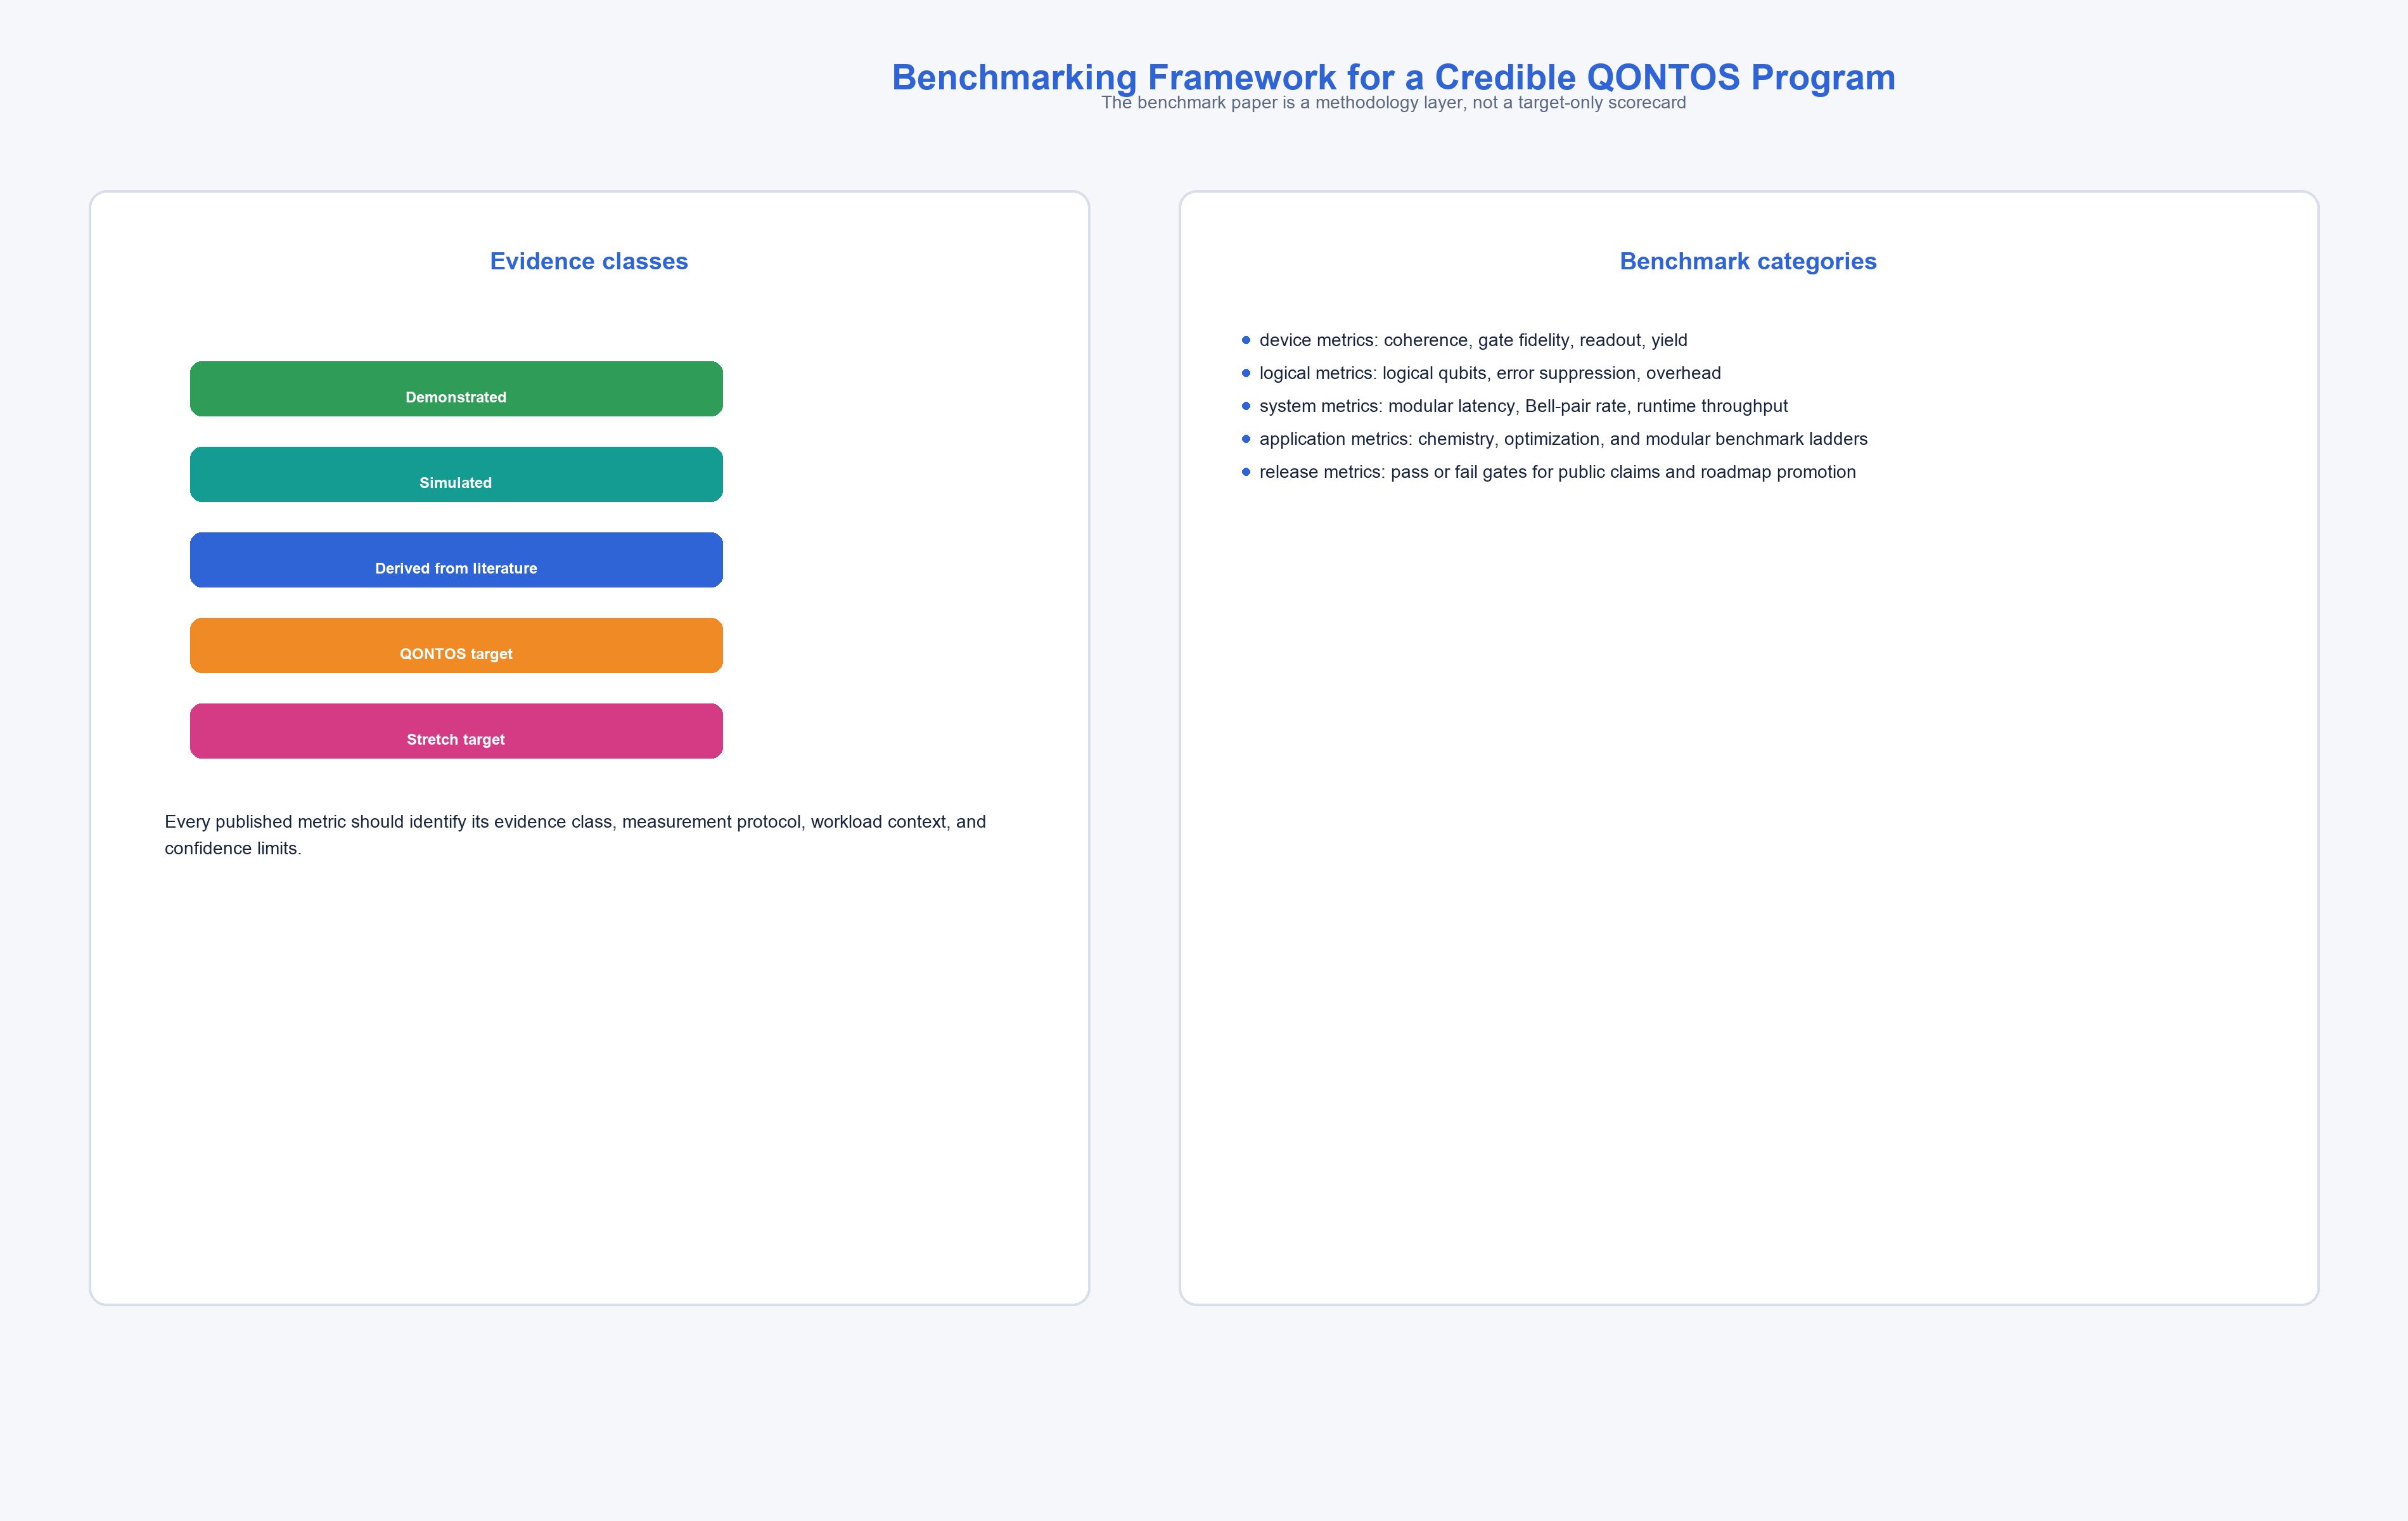
\includegraphics[width=\columnwidth]{../../figures/09_benchmarking.png}
\caption{Benchmark Evidence Pyramid.}
\label{fig:benchmark_pyramid}
\end{figure}

\subsection{Layer Definitions}

QONTOS organizes benchmarks into four layers reflecting the maturity of the execution environment. Because QONTOS builds a hybrid superconducting-photonic modular architecture---combining high-coherence tantalum-on-silicon transmon qubits (Paper~02) with photonic interconnects for inter-module entanglement distribution (Paper~04)---the benchmark framework must capture performance along both the superconducting device axis and the photonic networking axis.

\begin{table}[H]
\centering
\caption{Benchmark layer definitions.}
\label{tab:layers}
\begin{tabular}{@{}l L{2cm} l L{2cm}@{}}
\toprule
\textbf{Layer} & \textbf{Environment} & \textbf{Evidence} & \textbf{Use} \\
\midrule
L0 & Simulator-backed pipeline & MEAS.-SIM. & Platform validation \\
L1 & Digital-twin runtime & DT-PROJ. & Architecture projections \\
L2 & Prototype HW & MEAS.-HW & Device characterization \\
L3 & Large-scale FT system & TARGET & Roadmap milestones \\
\bottomrule
\end{tabular}
\end{table}

\textbf{Layer promotion rule.} A metric may only advance from a lower layer to a higher layer when the evidence requirements of the higher layer are fully satisfied. A digital-twin projection (L1) does not become a hardware result (L2) merely by asserting that the noise model is realistic. Hardware measurement on a calibrated device with raw data is required.

\subsection{Benchmark Protocol Specification}

Each benchmark in the \texttt{qontos-benchmarks} repository is defined by a protocol file. For example, the Quantum Volume protocol (QV-STANDARD-001) specifies:

\begin{enumerate}[leftmargin=*]
\item Select target width $d$.
\item Generate $N \geq 100$ random SU(4) circuits of depth $d$ on $d$ qubits.
\item For each circuit, compute the ideal heavy-output set classically.
\item Execute each circuit on the target backend with $S \geq 100$ shots.
\item Compute the heavy-output fraction $h_i$ for each circuit.
\item Compute $\bar{h} = (1/N) \sum h_i$.
\item Apply one-sided binomial test: reject $H_0$ ($\bar{h} \leq 2/3$) at $\alpha = 0.023$.
\item Report $\mathrm{QV} = 2^d$ if test passes; otherwise report $\mathrm{QV} < 2^d$.
\end{enumerate}

Pass threshold: $\bar{h} > 2/3$ with 97.7\% confidence. Confidence interval: 95\% bootstrap CI over $N$ circuits.

\textbf{[CLAIM-METHODOLOGY]} This protocol format is mandatory for all benchmarks. The \texttt{qontos-benchmarks} repository contains the reference implementation of every protocol defined in this paper.

\subsection{Modular-System Benchmarking}

Modular quantum architectures introduce benchmark challenges absent from monolithic systems. In the QONTOS hybrid superconducting-photonic platform, cross-module metrics are as critical as intra-module metrics. Martiel et al.\ (2021)~\cite{martiel2021} identified coprocessor-level benchmarking as a distinct problem requiring metrics that capture inter-module communication overhead.

\textbf{[CLAIM-METHODOLOGY]} QONTOS defines the following modular-system benchmark extensions:

\textbf{Inter-module gate fidelity.} Measured via IRB (Magesan et al.\ 2012~\cite{magesan2012}) applied specifically to entangling gates that span module boundaries.

\textbf{Modular Quantum Volume (MQV).} Extension of the QV protocol where the $d$-qubit register is distributed across $k$ modules. MQV is reported as a pair $(\mathrm{QV}_\mathrm{value}, k_\mathrm{modules})$.

\textbf{Distributed CLOPS (D-CLOPS).} Extension of CLOPS where circuit layers include inter-module communication steps. D-CLOPS is always reported alongside monolithic CLOPS on the same workload.

\textbf{Cross-module entanglement rate.} The number of Bell pairs generated per second across a module boundary, measured with full tomographic verification.

\textbf{Module-aware circuit partitioning overhead.} The ratio of total two-qubit gates after partitioning to the minimum two-qubit gate count on an all-to-all connected ideal machine.

\section{Baseline Comparisons and Gating Thresholds}

\subsection{Three Mandatory Baselines}

\textbf{[CLAIM-METHODOLOGY]} Every benchmark result at any layer must be reported alongside at least one of the following baselines. L2 and L3 results require all three.

\textbf{Ideal simulator baseline.} The benchmark is executed on a noiseless statevector or tensor-network simulator with the same circuit, qubit count, and measurement configuration.

\textbf{Noisy baseline.} The benchmark is executed on a standardized noise model: symmetric depolarizing noise at error rate $p = 10^{-3}$ per single-qubit gate and $p = 10^{-2}$ per two-qubit gate, with $T_1 = 100$~\textmu s and $T_2 = 100$~\textmu s relaxation.

\textbf{Digital-twin baseline.} The benchmark is executed on a calibrated noise model derived from the most recent hardware characterization data.

\subsection{Baseline Comparison Protocol}

Results must be presented in the following tabular format:

\begin{table}[H]
\centering
\caption{Baseline comparison format.}
\label{tab:baseline_comparison}
\begin{tabular}{@{}l l l l l l@{}}
\toprule
\textbf{Metric} & \textbf{Ideal} & \textbf{Noisy} & \textbf{DT} & \textbf{Meas.} & \textbf{Label} \\
\midrule
QV ($d{=}5$) & 32 & 32 & 32 & --- & MEAS.-SIM. \\
QV ($d{=}10$) & 1024 & 256 & 512 & --- & DT-PROJ. \\
CLOPS & --- & --- & --- & --- & TARGET \\
\bottomrule
\end{tabular}
\end{table}

\textbf{[CLAIM-METHODOLOGY]} The ``Measured Value'' column remains empty (``---'') until a hardware measurement is obtained. Under no circumstances may a digital-twin projection be placed in the ``Measured Value'' column.

\subsection{Pass/Fail Thresholds}

Each benchmark layer has explicit gating thresholds.

\textbf{Layer L0 gates:}

\begin{table}[H]
\centering
\caption{Layer L0 gating thresholds.}
\begin{tabular}{@{}l L{3cm} L{3cm}@{}}
\toprule
\textbf{Gate} & \textbf{Requirement} & \textbf{Pass Criterion} \\
\midrule
G0-1 & Protocol implemented & Protocol file exists, tests pass \\
G0-2 & Ideal baseline correct & Deviation $< 3\sigma$ from theory \\
G0-3 & Noisy baseline expected & Within analytic bound $\pm 10\%$ \\
G0-4 & Fully reproducible & Re-execution within CI \\
\bottomrule
\end{tabular}
\end{table}

\textbf{Layer L1 gates:}

\begin{table}[H]
\centering
\caption{Layer L1 gating thresholds.}
\begin{tabular}{@{}l L{3cm} L{3cm}@{}}
\toprule
\textbf{Gate} & \textbf{Requirement} & \textbf{Pass Criterion} \\
\midrule
G1-1 & All L0 gates passed & Documented \\
G1-2 & Noise model sourced & Provenance documented \\
G1-3 & Modular assumptions stated & Module count, topology recorded \\
G1-4 & DT bounded by baselines & ideal $\geq$ DT $\geq$ noisy \\
\bottomrule
\end{tabular}
\end{table}

\textbf{Layer L2 gates:}

\begin{table}[H]
\centering
\caption{Layer L2 gating thresholds.}
\begin{tabular}{@{}l L{3cm} L{3cm}@{}}
\toprule
\textbf{Gate} & \textbf{Requirement} & \textbf{Pass Criterion} \\
\midrule
G2-1 & All L1 gates passed & Documented \\
G2-2 & HW calibration available & Within 24 hours \\
G2-3 & Raw data archived & Data hash recorded \\
G2-4 & Consistent with DT & Within $3\sigma$ or explained \\
\bottomrule
\end{tabular}
\end{table}

\textbf{Layer L3 gates:}

\begin{table}[H]
\centering
\caption{Layer L3 gating thresholds.}
\begin{tabular}{@{}l L{3cm} L{3cm}@{}}
\toprule
\textbf{Gate} & \textbf{Requirement} & \textbf{Pass Criterion} \\
\midrule
G3-1 & All L2 gates passed per module & Documented per module \\
G3-2 & Modular benchmarks reported & MQV, D-CLOPS present \\
G3-3 & Application benchmark done & Above current validated level \\
G3-4 & FT overhead measured & Decoder latency included \\
\bottomrule
\end{tabular}
\end{table}

\section{Current QONTOS Benchmark Surface}

\subsection{Current Benchmark Harness}

\textbf{[CLAIM-MEASURED-SIMULATOR]} The QONTOS benchmark harness is implemented in the \texttt{qontos-benchmarks} repository and currently supports the following capabilities:

\begin{table}[H]
\centering
\caption{Current benchmark harness status.}
\label{tab:harness}
\begin{tabular}{@{}l l@{}}
\toprule
\textbf{Capability} & \textbf{Status} \\
\midrule
Randomized benchmarking (RB)~\cite{knill2008} & Implemented \\
Interleaved RB~\cite{magesan2012} & Implemented \\
Quantum Volume~\cite{cross2019} & Implemented \\
CLOPS~\cite{wack2021} & Implemented \\
Application benchmarks (H$_2$, LiH)~\cite{lubinski2023} & Implemented \\
Small QAOA benchmarks & Implemented \\
Modular QV (MQV) & In development \\
Distributed CLOPS & In development \\
SupermarQ feature extraction~\cite{tomesh2022} & Planned \\
\bottomrule
\end{tabular}
\end{table}

\textbf{Execution environments currently supported:}

\begin{itemize}[leftmargin=*]
\item \textbf{Statevector simulator:} Ideal noiseless execution for baseline generation. Up to 30 qubits on standard hardware, up to 40 qubits on high-memory nodes.
\item \textbf{Noisy simulator:} Depolarizing and relaxation noise models with configurable parameters.
\item \textbf{Digital-twin runtime:} Modular architecture simulator with configurable module count, topology, inter-module gate fidelity, and classical communication latency.
\end{itemize}

\subsection{Benchmark Report Format}

Every benchmark execution produces a structured report containing the report ID, benchmark ID, execution timestamp, software version, environment, configuration hash, baselines (ideal, noisy, digital-twin), result with confidence interval, claim label, and gates passed/failed.

\section{Application Benchmark Ladder}

\textbf{[CLAIM-METHODOLOGY]} QONTOS benchmarks application-level progress using graduated workload ladders rather than a single flagship endpoint.

\subsection{Chemistry Ladder}

\begin{table}[H]
\centering
\caption{Chemistry application benchmark ladder.}
\label{tab:chem_ladder}
\begin{tabular}{@{}l l l l l@{}}
\toprule
\textbf{Rung} & \textbf{Workload} & \textbf{Qubits} & \textbf{Threshold} & \textbf{Claim} \\
\midrule
C1 & H$_2$ ground state & 2--4 & $<$1.6~mHa & MEAS.-SIM. \\
C2 & LiH dissociation & 6--12 & $<$1.6~mHa & MEAS.-SIM. \\
C3 & Small catalysts & 20--40 & $<$4~mHa & DT-PROJ. \\
C4 & Medium catalysts & 50--100 & $<$10~mHa & TARGET \\
C5 & FeMoco-class & 100--200 & $<$1.6~mHa & STRETCH \\
\bottomrule
\end{tabular}
\end{table}

\textbf{[CLAIM-METHODOLOGY]} FeMoco (rung~C5) remains the flagship stretch benchmark, but no QONTOS communication may reference FeMoco without also reporting current validated performance on rungs~C1 and~C2.

\subsection{Optimization Ladder}

\begin{table}[H]
\centering
\caption{Optimization application benchmark ladder.}
\label{tab:opt_ladder}
\begin{tabular}{@{}l l l l l@{}}
\toprule
\textbf{Rung} & \textbf{Workload} & \textbf{Qubits} & \textbf{Threshold} & \textbf{Claim} \\
\midrule
O1 & MaxCut ($n \leq 16$) & 8--16 & Ratio $> 0.8$ & MEAS.-SIM. \\
O2 & Portfolio opt. & 15--30 & Within 5\% & DT-PROJ. \\
O3 & Vehicle routing & 50--100 & Competitive TTS & TARGET \\
O4 & Large-scale & 1000+ & Measurable adv. & STRETCH \\
\bottomrule
\end{tabular}
\end{table}

\subsection{Simulation Ladder}

\begin{table}[H]
\centering
\caption{Simulation application benchmark ladder.}
\label{tab:sim_ladder}
\begin{tabular}{@{}l l l l l@{}}
\toprule
\textbf{Rung} & \textbf{Workload} & \textbf{Qubits} & \textbf{Threshold} & \textbf{Claim} \\
\midrule
S1 & Ising dynamics & 10--20 & $F > 0.95$ & MEAS.-SIM. \\
S2 & Heisenberg & 25--50 & Error $< 5\%$ & DT-PROJ. \\
S3 & Lattice gauge & 100+ & Controlled err. & STRETCH \\
\bottomrule
\end{tabular}
\end{table}

\subsection{Flagship Benchmark Rule}

\textbf{[CLAIM-METHODOLOGY]} No flagship benchmark (C5, O4, S3) may appear in any QONTOS communication without: (1)~current validated rung on the same ladder, (2)~number of rungs between current capability and the flagship, (3)~explicit list of requirements for each intermediate rung, and (4)~estimated timeline with uncertainty range.

\section{System-Level Metric Definitions}

\subsection{Gate-Level Metrics}

\begin{table}[H]
\centering
\caption{Gate-level metric definitions.}
\begin{tabular}{@{}l l l@{}}
\toprule
\textbf{Metric} & \textbf{Protocol} & \textbf{Reference} \\
\midrule
1Q gate error & Standard RB & Knill et al.~\cite{knill2008} \\
2Q gate error & IRB & Magesan et al.~\cite{magesan2012} \\
Cross-module gate error & IRB (modular) & Magesan et al.~\cite{magesan2012} \\
SPAM error & Dedicated protocol & Knill et al.~\cite{knill2008} \\
\bottomrule
\end{tabular}
\end{table}

\subsection{System-Level Metrics}

\begin{table}[H]
\centering
\caption{System-level metric definitions.}
\begin{tabular}{@{}l l l@{}}
\toprule
\textbf{Metric} & \textbf{Protocol} & \textbf{Reference} \\
\midrule
Quantum Volume & Heavy-output test & Cross et al.~\cite{cross2019} \\
Modular QV & Distributed test & This paper \\
CLOPS & QV-layer throughput & Wack et al.~\cite{wack2021} \\
D-CLOPS & Modular throughput & This paper \\
\bottomrule
\end{tabular}
\end{table}

\subsection{Logical-Qubit Metrics}

\textbf{[CLAIM-METHODOLOGY]} A logical qubit is counted as usable only when all of the following are specified: (1)~error-correcting code family, (2)~code distance and physical-to-logical ratio, (3)~decoder type and latency, (4)~logical error rate per cycle with cycle duration, and (5)~correction cycle budget for the target computation.

\begin{table}[H]
\centering
\caption{Logical-qubit metric targets.}
\label{tab:logical_metrics}
\begin{tabular}{@{}l l l l@{}}
\toprule
\textbf{Metric} & \textbf{Base} & \textbf{Aggressive} & \textbf{Stretch} \\
\midrule
Phys.-to-logical ratio & 1000:1 & 300:1 & 100:1 \\
Logical error rate & $10^{-4}$/cycle & $10^{-6}$/cycle & $10^{-8}$/cycle \\
Decoder latency & $< 1$~\textmu s & $< 0.5$~\textmu s & $< 0.1$~\textmu s \\
Logical qubit count & 1--20 & 100--1,000 & 10,000+ \\
\bottomrule
\end{tabular}
\end{table}

\subsection{Scenario Targets (System Level)}

\textbf{[CLAIM-QONTOS-TARGET / STRETCH-TARGET]}

\begin{table}[H]
\centering
\caption{System-level scenario targets.}
\label{tab:scenario_targets}
\begin{tabular}{@{}l l l l l@{}}
\toprule
\textbf{Metric} & \textbf{L0} & \textbf{L1} & \textbf{L2} & \textbf{L3} \\
\midrule
QV & Sim. & $2^{10}$--$2^{15}$ & $2^{15}$--$2^{20}$ & $2^{20}$+ \\
CLOPS & Sim. & $10^3$--$10^5$ & $10^5$--$10^8$ & $10^8$--$10^{12}$ \\
Logical qubits & N/A & 1--20 & 100--1,000 & 10,000+ \\
Bell rate & N/A & $10^3$/s & $10^6$/s & $10^9$/s \\
Circuit depth & $10^3$ & $10^4$ & $10^6$ & $10^{12}$ \\
\bottomrule
\end{tabular}
\end{table}

\section{Confidence Interval and Statistical Reporting}

\subsection{Mandatory Statistical Requirements}

\textbf{[CLAIM-METHODOLOGY]} All benchmark results must report uncertainty using the following conventions:

\begin{enumerate}[leftmargin=*]
\item \textbf{Quantum Volume:} One-sided binomial test at $\alpha = 0.023$ (97.7\% confidence), per Cross et al.\ (2019)~\cite{cross2019}. Additionally report the 95\% bootstrap CI for the mean heavy-output fraction.
\item \textbf{CLOPS:} Report mean and standard deviation over at least 10 independent executions. Report 95\% CI using the $t$-distribution.
\item \textbf{Gate fidelity (RB/IRB):} Report the fit uncertainty from the exponential decay model. Use at least 30 random sequences per sequence length and at least 6 sequence lengths. Report 95\% CI on the error-per-gate parameter.
\item \textbf{Application benchmarks:} Report the mean and 95\% CI of the figure of merit over at least 10 independent runs with different random seeds or shot allocations.
\end{enumerate}

\subsection{Significance Testing for Improvement Claims}

\textbf{[CLAIM-METHODOLOGY]} Any claim that a new QONTOS version, algorithm, or hardware configuration improves benchmark performance must be supported by a two-sided hypothesis test at the $\alpha = 0.05$ significance level. The test must account for multiple comparisons if more than one metric is simultaneously evaluated (Bonferroni correction or equivalent).

\section{Release and Communication Gating}

\subsection{Benchmark Maturity Levels}

\begin{table}[H]
\centering
\caption{Benchmark maturity levels.}
\begin{tabular}{@{}l l L{4cm}@{}}
\toprule
\textbf{Stage} & \textbf{Name} & \textbf{Requirements} \\
\midrule
M0 & Protocol draft & Protocol file written; not implemented \\
M1 & Harness implemented & Code in repo; unit tests pass \\
M2 & Baselines validated & All baselines produce expected results \\
M3 & Report generated & All metadata fields populated \\
M4 & Peer reviewed & Reviewed by non-involved team member \\
M5 & Publication ready & All gates passed; archived with hash \\
\bottomrule
\end{tabular}
\end{table}

\subsection{Safe Communication Language}

The following language is pre-approved for external communication:

\begin{itemize}[leftmargin=*]
\item ``QONTOS has \textbf{measured} [metric] on its simulator-backed pipeline''---requires M5, MEASURED-SIMULATOR.
\item ``QONTOS \textbf{projects} [metric] under [assumptions] using its digital twin''---requires M5, DIGITAL-TWIN-PROJECTION.
\item ``QONTOS \textbf{targets} [metric] for its [timeline] modular architecture''---requires M3, QONTOS-TARGET.
\item ``QONTOS has defined a \textbf{stretch target} of [metric] requiring [breakthroughs]''---requires M3, STRETCH-TARGET.
\end{itemize}

\subsection{Prohibited Communication Language}

The following formulations are prohibited unless the corresponding MEASURED-HARDWARE result at M5 exists: ``QONTOS achieves Quantum Volume X,'' ``QONTOS demonstrates CLOPS of Y,'' ``QONTOS has Z logical qubits operational,'' ``QONTOS demonstrates quantum advantage,'' ``QONTOS outperforms [competitor] on [benchmark].''

\section{Connection to the QONTOS Paper Series}

This benchmarking framework provides the validation backbone for every companion paper:

\begin{table}[H]
\centering
\caption{Paper series benchmark connections.}
\label{tab:paper_connections}
\begin{tabular}{@{}l L{5.5cm}@{}}
\toprule
\textbf{Paper} & \textbf{Key Claims Validated Here} \\
\midrule
01: Architecture & Module count targets, inter-module fidelity \\
02: Ta--Si Qubits & Gate fidelity, $T_1$/$T_2$ protocols \\
03: Error Correction & Logical error rate, overhead ratios \\
04: Photonic Links & Cross-module Bell rate, gate fidelity \\
05: AI Decoding & Decoder latency, logical error rate \\
06: Software Stack & CLOPS, partitioning overhead \\
07: Cryogentic Infra. & HW calibration for digital-twin baselines \\
08: Algorithms & Application benchmark ladder \\
10: Roadmap 2030 & Scenario targets, milestone gating \\
\bottomrule
\end{tabular}
\end{table}

\textbf{[CLAIM-METHODOLOGY]} If a claim in any companion paper cannot be traced to a benchmark definition, measurement condition, or validation gate in this paper, that claim must carry the UNVALIDATED label.

\section{Conclusion}

Benchmarking is not a post-hoc validation exercise---it is the structural foundation on which every QONTOS claim stands or falls. This paper has established:

\begin{enumerate}[leftmargin=*]
\item A \textbf{claim-label taxonomy} (Section~1.2) that forces every metric to declare its evidence basis.
\item \textbf{Rigorous benchmark definitions} (Section~1.3) grounded in peer-reviewed protocols from Knill et al.~\cite{knill2008}, Magesan et al.~\cite{magesan2012}, Cross et al.~\cite{cross2019}, Wack et al.~\cite{wack2021}, Lubinski et al.~\cite{lubinski2023}, and Tomesh et al.~\cite{tomesh2022}.
\item \textbf{Mandatory measurement conditions} (Section~1.4) ensuring reproducibility.
\item \textbf{Modular-system extensions} (Section~2.3) including MQV and D-CLOPS.
\item \textbf{Three mandatory baselines} (Section~3.1) against which every result must be compared.
\item \textbf{Explicit pass/fail gates} (Section~3.3) preventing premature promotion.
\item \textbf{Application benchmark ladders} (Section~5) ensuring visibility of the gap to flagship targets.
\item \textbf{Statistical reporting requirements} (Section~7) including confidence intervals and significance testing.
\item \textbf{Communication gating} (Section~8) preventing unsafe language.
\end{enumerate}

The most important contribution is the structural discipline: every claim maps to a protocol, every protocol maps to an implementation, every implementation produces baselines, and every result carries a confidence interval and a claim label.

\textbf{[CLAIM-METHODOLOGY]} All benchmark protocols, harness code, baseline configurations, and report templates are maintained in the \texttt{qontos-benchmarks} repository. This paper and the repository evolve together.

\begin{thebibliography}{9}

\bibitem{cross2019}
A.~W.~Cross, L.~S.~Bishop, S.~Sheldon, P.~D.~Nation, and J.~M.~Gambetta,
``Validating quantum computers using randomized model circuits,''
\textit{Phys.\ Rev.\ A}, vol.~100, p.~032328, 2019.

\bibitem{magesan2012}
E.~Magesan, J.~M.~Gambetta, and J.~Emerson,
``Efficient measurement of quantum gate error by interleaved randomized benchmarking,''
\textit{Phys.\ Rev.\ Lett.}, vol.~109, p.~080505, 2012.

\bibitem{knill2008}
E.~Knill \textit{et al.},
``Randomized benchmarking of quantum gates,''
\textit{Phys.\ Rev.\ A}, vol.~77, p.~012307, 2008.

\bibitem{proctor2022}
T.~Proctor, K.~Rudinger, K.~Young, E.~Nielsen, and R.~Blume-Kohout,
``Measuring the capabilities of quantum computers,''
\textit{Nature Phys.}, vol.~18, pp.~75--79, 2022.

\bibitem{lubinski2023}
T.~Lubinski \textit{et al.},
``Application-oriented performance benchmarks for quantum computing,''
\textit{IEEE Trans.\ Quantum Eng.}, vol.~4, p.~3100332, 2023.

\bibitem{ibm2024}
IBM Quantum,
``Quantum Volume,''
IBM Quantum documentation, 2024.

\bibitem{wack2021}
A.~Wack \textit{et al.},
``Quality, speed, and scale: Three key attributes to measure the performance of near-term quantum computers,''
arXiv:2110.14108, 2021.

\bibitem{tomesh2022}
T.~Tomesh \textit{et al.},
``SupermarQ: A scalable quantum benchmark framework,''
in \textit{Proc.\ IEEE HPCA}, 2022.

\bibitem{martiel2021}
S.~Martiel, T.~Ayral, and C.~Allouche,
``Benchmarking quantum coprocessors in an application-centric, hardware-agnostic, and scalable way,''
arXiv:2104.10698, 2021.

\end{thebibliography}

\end{document}
